%% Sect. 3 -- from augur_AMT_§2.9_3 draft v1 (2026-09-21, Fig. 3 sentences of 2026-09-27)
\section{Verification}
\label{sec:3}

Five things are verified, and they are different things. That the
implementation solves the equations of Sect.~\ref{sec:2}; that the analytic Jacobian is the
derivative it claims to be; that an independent implementation of the same
problem returns the same answer; that the diagnostics of Sects.~\ref{sec:4} and \ref{sec:5} measure
what they are said to measure, on data whose truth is known; and that the two
hot channels share a relative scale. Absolute concentration accuracy against a
reference standard is not established here and is not claimed anywhere in this
paper.

Results in Sects.~\ref{sec:3}--\ref{sec:6} are reported for three retrieval configurations taken
from the field case of Sect.~\ref{sec:7} and labelled by the cells they come from. What
distinguishes them for the retrieval is listed in Table~\ref{tab:1}: the fitting window,
the order of the baseline polynomial, the permitted shift range and the light
level; the full configuration is in Appendix~\ref{app:A}. None of the results in Sects.~\ref{sec:3}--\ref{sec:6} depends on the chemistry the cells
measure; where a result depends on a property of a configuration, that property
is named. Figure~\ref{fig:2} shows one record retrieved in all three configurations.

\begin{table}[t]
\caption{Retrieval configurations used in Sects.~\ref{sec:3}--\ref{sec:6}, in short form; windows are rounded to the nanometre, and the full configuration, including the exact window bounds, is in Table~\ref{tab:config}.}
\label{tab:1}
\begin{tabular}{llllll}
\tophline
Label & Cell & Window (nm) & Baseline & Shift range (px) & Light level \\
\middlehline
hot ANs & 300\,$^{\circ}$C & 430--462 & 4th order & $-10$ to $0.5$ & nominal \\
hot PNs & 180\,$^{\circ}$C & 444--471 & 3rd order & $-5$ to $5$ & nominal \\
cold & ambient & 438--476 & 4th order & fixed at $-0.5$ & reduced \\
\bottomhline
\end{tabular}
\end{table}

\begin{figure*}[p]
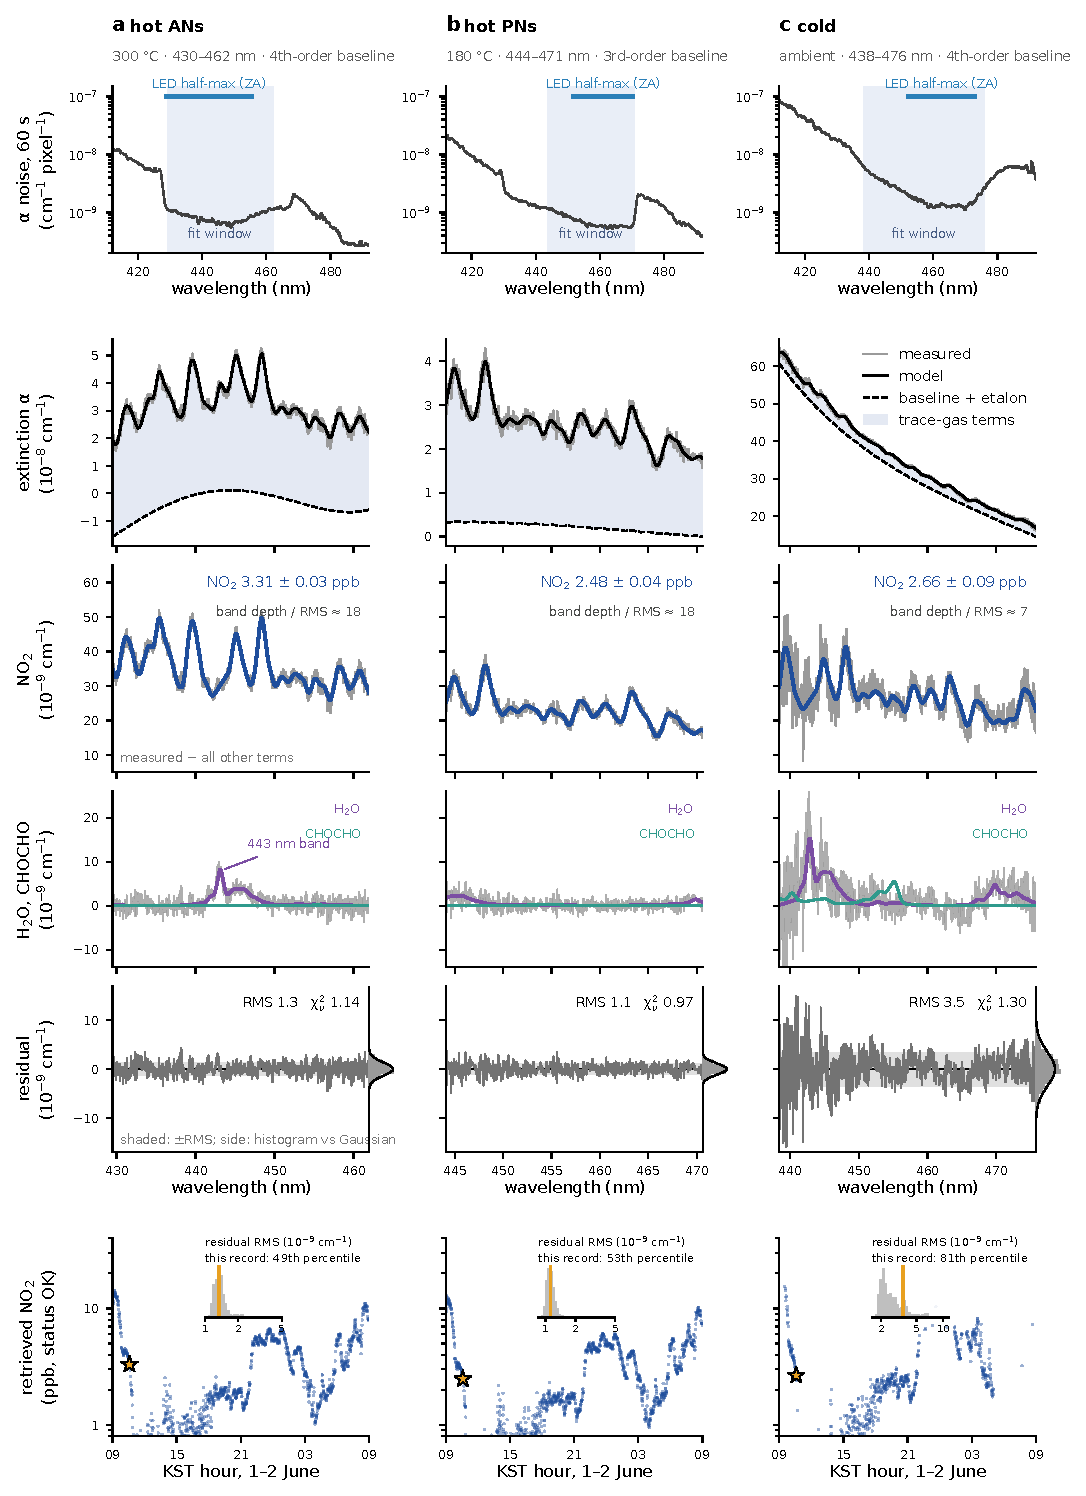
\includegraphics[width=\textwidth,height=0.66\textheight,keepaspectratio]{figures/fig02.pdf}
\caption{One record (1 June 2026, 10:35 KST; cold channel 10:34:34) retrieved in the three
configurations of Table~\ref{tab:1}. Columns: \textbf{(a)} hot ANs (300\,$^{\circ}$C), \textbf{(b)} hot PNs (180\,$^{\circ}$C), \textbf{(c)} cold.
\textbf{Top row:} per-pixel noise of the 60\,s extinction spectrum in the hour around the record, with the fit window
shaded. Each window sits on the low-noise band set by its LED (bar: LED emission half-maximum from zero-air
spectra); the cold window extends 13\,nm below its LED half-maximum, where the noise is several times higher; the step at 428\,nm in (a) is the band-pass filter edge and the step at 470\,nm in (b) is the
red edge of the 469\,nm LED. \textbf{Middle block,} top to bottom: measured extinction with the fitted model and the
baseline-plus-etalon term (shading: sum of trace-gas terms); the NO$_2$ contribution, shown as the measurement minus
every other fitted term, with the fitted NO$_2$ term; the same for H$_2$O, with the fitted CHOCHO term; and the
residual, with $\pm$RMS shaded and its histogram against a Gaussian of the same RMS at right. The lower three rows share
one vertical scale across columns. Values in the NO$_2$ row are the operational retrieval and its reported 1$\sigma$;
``band depth / RMS'' is the peak-to-peak of the fitted NO$_2$ term divided by the residual RMS. \textbf{Bottom row:}
the NO$_2$ retrieved by the same configuration over the surrounding 24\,h (fits with reduced $\chi^2 \le 1.5$; $n = \fieldnum{1397}$, \fieldnum{1399}, \fieldnum{707}),
the star marking this record; inset: distribution of residual RMS over those fits, on which this record sits at the
\fieldnum{49}th, \fieldnum{53}rd and \fieldnum{81}st percentile.}
\label{fig:2}
\end{figure*}

\subsection{Recovery of a known truth}
\label{sec:3.1}

Spectra are generated from the forward model of Sect.~\ref{sec:2.1} with prescribed gas
amounts, a Chebyshev baseline, a wavelength shift and a squeeze, and retrieved
with the same model. Over 27 combinations -- nine shifts from $-4$ to $+4$\,px (including sub-pixel
values of $\pm0.37$\,px) crossed with squeezes of 0.998, 1.000 and 1.002 -- the largest error in the retrieved NO$_2$ amount is
$9.5\times10^{-13}$ relative and the largest error in the recovered shift $6.7\times10^{-10}$\,px. The
retrieval reproduces its own forward model to machine precision, which is a
statement about the solver and not about the instrument.

The baseline order is the one structural choice the retrieval makes on its
own. Sweeping it from 0 to 8 on a noise-free spectrum built with a
fourth-order baseline, the retrieved NO$_2$ is in error by 27\,\% at order 0 and
0.75\,\% at order 1, and reaches machine precision at order 2 and above; the
normalised condition number rises from 14.9 to 33.8 across the sweep and the
degrees of freedom fall from 543 to 535. On noisy realisations of the same
spectrum the scatter of the retrieved NO$_2$ is 0.88 to 0.91 times the reported
1$\sigma$ at order 2 and above. For this configuration, with white photon noise and a correct model, the
reported uncertainty is accurate to about ten per cent -- which is the
baseline against which the structural terms of Sect.~\ref{sec:4} should be read (Fig.~\ref{fig:3}a, b). It is a
statement about one configuration: across the 13 synthetic instruments of Fig.~\ref{fig:1}a the white-noise ratio
ranges from 0.91 to 1.32, and at nominal noise it lies between 1.22 and 1.32 in 9 of them, where the free
wavelength shift adds scatter the covariance does not carry (Sect.~\ref{sec:3.4}).

\begin{figure*}[t]
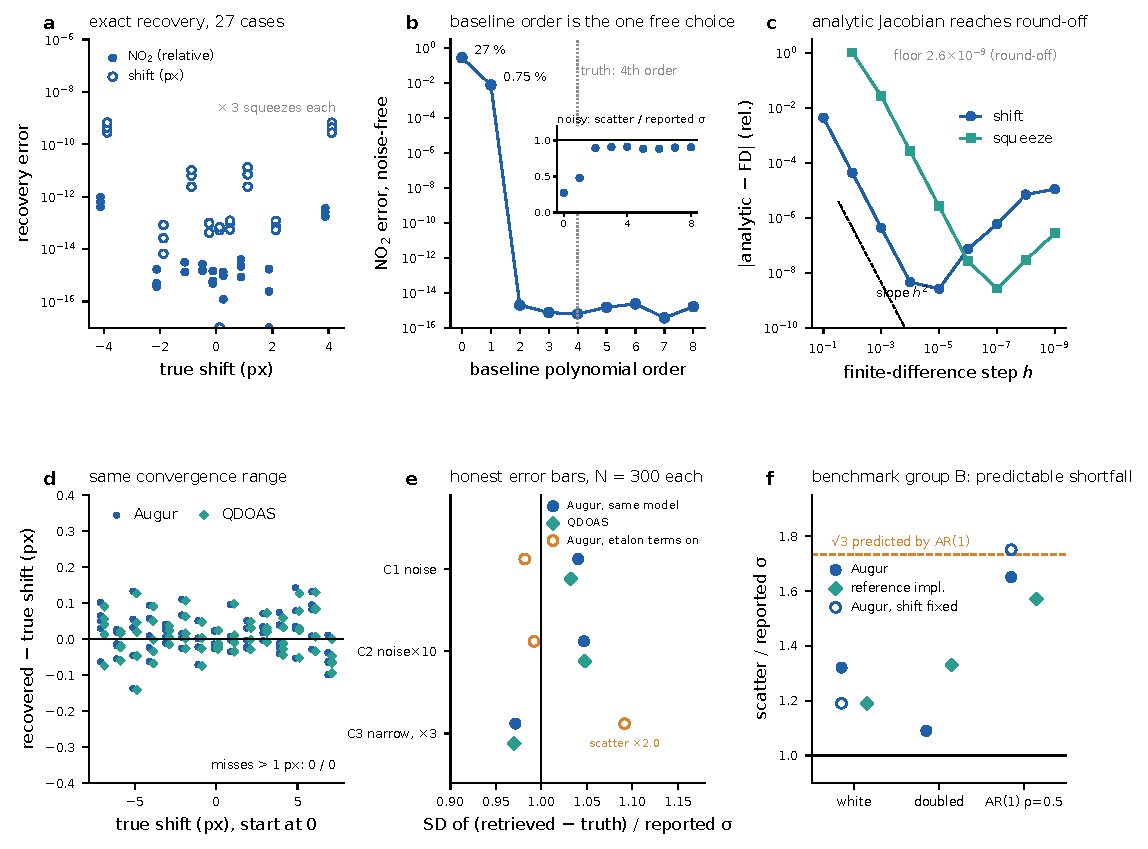
\includegraphics[width=\textwidth]{figures/fig03.pdf}
\caption{Validation of the retrieval core. \textbf{(a)} Error in the recovered NO$_2$ amount (filled, relative) and
wavelength shift (open, px) for 27 noise-free spectra: nine shifts between $-4$ and $+4$\,px, each with squeezes 0.998, 1.000
and 1.002. \textbf{(b)} Error in NO$_2$ against the order of the fitted baseline for a noise-free spectrum built with a
fourth-order baseline; inset, on noisy realisations of the same spectrum, the realised scatter of NO$_2$ divided by the
reported 1$\sigma$. \textbf{(c)} Difference between the analytic Golub--Pereyra Jacobian and a central finite difference of the
projected residual, against the finite-difference step, for the shift and the squeeze; the dashed line has slope $h^2$.
\textbf{(d)} Shift recovered by Augur and by QDOAS minus the true shift, for true shifts from $-7$ to $+7$\,px (five noisy
realisations each, both started at 0). \textbf{(e)} Standard deviation of (retrieved $-$ true)/reported $\sigma$ over 300 realisations
in each of three conditions (measurement noise; ten times that; a narrow window with three times the noise), for Augur
and QDOAS fitting the same model, and for Augur with its etalon terms switched on. \textbf{(f)} Benchmark group B: realised
scatter divided by the reported uncertainty under white, doubled and autocorrelated (AR(1), $\rho = 0.5$) noise, for Augur,
for the benchmark's reference implementation and for Augur with the shift fixed at its true value; the dashed line is the
$\sqrt{3}$ inflation predicted for $\rho = 0.5$.}
\label{fig:3}
\end{figure*}

\subsection{The analytic Jacobian}
\label{sec:3.2}

The two-term Golub--Pereyra derivative of Sect.~\ref{sec:2.3} is compared against a central
finite difference of the projected residual, evaluated inside a real fit
rather than on a constructed test function: the optimiser call is intercepted
and the analytic Jacobian it was handed is differenced against the residual it
was minimising. An invariant check of this form runs on every fit in the test
suite at the solver's default step; what is reported here is the step-size
sweep (Table~\ref{tab:jacobian_steps}), which is what turns a passing check into a measurement.

\begin{table}[t]
\caption{Difference between the analytic Golub--Pereyra Jacobian and a central finite difference of the projected residual, evaluated inside a real fit, against the finite-difference step $h$, for the shift (px) and the squeeze. Bold: the minimum of each column.}
\label{tab:jacobian_steps}
\begin{tabular}{lll}
\tophline
step $h$ & shift (px) & squeeze \\
\middlehline
$10^{-1}$ & $4.31\times10^{-3}$ & outside the box \\
$10^{-2}$ & $4.29\times10^{-5}$ & 1.02 \\
$10^{-3}$ & $4.29\times10^{-7}$ & $2.63\times10^{-2}$ \\
$10^{-4}$ & $4.51\times10^{-9}$ & $2.61\times10^{-4}$ \\
$10^{-5}$ & $\mathbf{2.60\times10^{-9}}$ & $2.61\times10^{-6}$ \\
$10^{-6}$ & $7.28\times10^{-8}$ & $2.61\times10^{-8}$ \\
$10^{-7}$ & $5.79\times10^{-7}$ & $\mathbf{2.64\times10^{-9}}$ \\
$10^{-8}$ & $6.95\times10^{-6}$ & $2.87\times10^{-8}$ \\
$10^{-9}$ & $1.09\times10^{-5}$ & $2.70\times10^{-7}$ \\
\bottomhline
\end{tabular}
\end{table}

Both parameters give the expected V (Fig.~\ref{fig:3}c). The truncation branch falls with a fitted
slope of $+2.001$ in each, which is the $h^2$ of a central difference, and the
round-off branch rises again as the difference of two nearly equal numbers
loses significance. The minima are $2.60\times10^{-9}$ for the shift and
$2.64\times10^{-9}$ for the squeeze, a ratio of 1.018: the two parameters reach
the same floor, which is the signature of a floor set by round-off in the
shared residual evaluation rather than by any error in either derivative.

This is a stronger statement than agreement at one step size. An analytic
expression that omitted a term -- the one-term approximation of \citet{Kaufman_1975}, which drops the derivative of the projector, is the natural candidate
-- would agree with the finite difference only down to the size of the omitted
term and would then flatten, not descend to the round-off floor. The descent
is what identifies the expression being differentiated as the derivative
itself.

The two parameters must be swept separately. The shift is measured in pixels
and is $O(1)$, while the squeeze is a multiplier near unity constrained to a
box of order $\pm 0.02$, so $h = 10^{-2}$ is already half the box for the
squeeze and the entry there is a bound artefact rather than a failure of the
derivative. A combined maximum over both parameters would show 1.02 at that
step and hide the V.

\subsection{An independent implementation of the same problem}
\label{sec:3.3}

QDOAS \citep{Danckaert_2017} solves the same separable least-squares problem by a
different route: Marquardt--Levenberg with a singular-value decomposition and a
numerically differenced Jacobian, against Augur's variable projection with an
analytic projected Jacobian. It does not know about cavities, so the
comparison is made by presenting the extinction spectrum as a virtual
transmission, $I = \exp(-K\alpha)$ with $I_0 = 1$, whereby the optical depth QDOAS
forms is exactly $K\alpha$ and the two codes are solving the same equations on
the same numbers.

On noise-free synthetic spectra with shifts of 0, $-1.96$, $+2$ and $-4$\,px, Augur
recovers NO$_2$ to $9.5\times10^{-13}$ relative and QDOAS to $5.0\times10^{-3}$, the latter limited by
its output resolution rather than by its algorithm; QDOAS recovers the shift
to within 0.0042\,px. On 30 noisy realisations the two codes have
root-mean-square relative errors of 0.0042 and 0.0045 against the same truth,
and differ from each other by at most $5.7\times10^{-3}$ relative in NO$_2$. On the field record (53 days), with each spectrum's measured temperature and pressure used
for the unit conversion and records selected by an NO$_2$-conditional $\chi^2$ envelope, the NO$_2$ amounts of the
two codes agree with $r^2 \ge \fieldnum{0.990}$ in all three configurations (Table~\ref{tab:qdoas_field}). The agreement is
not a scale identity: the Deming slope QDOAS/Augur is \fieldnum{1.039} in the cold configuration and \fieldnum{1.063} and
\fieldnum{1.043} in the 180 and 300\,$^{\circ}$C configurations, where $r^2 = \fieldnum{1.000}$, so the two codes differ in the
heated-channel NO$_2$ scale by \fieldnum{4}--\fieldnum{6}\,\% for a reason we have not identified. The weak absorbers agree less
well (CHOCHO $r^2$ \fieldnum{0.889}--\fieldnum{0.959}, slope \fieldnum{0.81}--\fieldnum{1.19}; H$_2$O slope \fieldnum{1.04}--\fieldnum{1.38}).

\begin{table}[t]
\caption{Agreement of QDOAS with Augur on the field record, per retrieval configuration and species: number of
records $n$ in the NO$_2$-conditional $\chi^2$ envelope, Deming slope QDOAS/Augur ($\lambda = 1$) and $r^2$. The
unit conversion uses each spectrum's measured temperature and pressure.}
\label{tab:qdoas_field}
\begin{tabular}{lllll}
\tophline
configuration & species & $n$ & Deming slope & $r^2$ \\
\middlehline
cold & NO$_2$ & \fieldnum{36\,241} & \fieldnum{1.039} & \fieldnum{0.990} \\
cold & CHOCHO & \fieldnum{36\,241} & \fieldnum{0.807} & \fieldnum{0.889} \\
cold & H$_2$O & \fieldnum{36\,241} & \fieldnum{1.377} & \fieldnum{0.887} \\
hot PNs (180\,$^{\circ}$C) & NO$_2$ & \fieldnum{73\,916} & \fieldnum{1.063} & \fieldnum{1.000} \\
hot PNs (180\,$^{\circ}$C) & CHOCHO & \fieldnum{73\,916} & \fieldnum{1.195} & \fieldnum{0.914} \\
hot PNs (180\,$^{\circ}$C) & H$_2$O & \fieldnum{73\,916} & \fieldnum{1.042} & \fieldnum{0.974} \\
hot ANs (300\,$^{\circ}$C) & NO$_2$ & \fieldnum{74\,539} & \fieldnum{1.043} & \fieldnum{1.000} \\
hot ANs (300\,$^{\circ}$C) & CHOCHO & \fieldnum{74\,539} & \fieldnum{1.054} & \fieldnum{0.959} \\
hot ANs (300\,$^{\circ}$C) & H$_2$O & \fieldnum{74\,539} & \fieldnum{1.038} & \fieldnum{0.981} \\
\bottomhline
\end{tabular}
\end{table}

In a
larger test with 300 realisations in each of three noise conditions, the
standard deviation of the error normalised by the reported uncertainty is 0.97
to 1.05 for both codes when they fit the same model, and started from zero both
recover true shifts between $-7$ and $+7$\,px with no miss larger than a pixel
(Fig.~\ref{fig:3}d, e). Switching on Augur's etalon terms in the narrow window doubles the
scatter there -- a choice of model, not a property of the solver.

The conclusion drawn from this in Sect.~\ref{sec:2.9} is therefore narrower than identity: on
synthetic spectra the two codes return the same concentrations, and on field spectra they agree in NO$_2$
to within a scale difference of a few per cent. Where they diverge most -- the wavelength shift in the cold
window, and with it the weak absorbers there (Sect.~\ref{sec:5.1}) -- the data do not determine the shift, so
neither code's value is established by its fit.

\subsection{A benchmark that others can run}
\label{sec:3.4}

The comparison of Sect.~\ref{sec:3.3} is specific to one pair of codes and one set of cross
sections. To make the same measurements repeatable elsewhere we release a
synthetic benchmark of 261 cases in six groups: exact recovery with no noise
(A), reported uncertainty against realised scatter under white, doubled and
autocorrelated noise (B), bias from a deliberately incomplete model (C), cases
whose wavelength shift is not determined by the data (D), the same truth
presented in two fitting windows (E), and the cost of the sub-pixel
interpolator against band-limited truth (F). Truth is known by construction,
the spectra are built from the instrument's own cross sections and wavelength
calibration but contain no retrieval code, and the generator is deterministic
under a stated seed.

Group B is worth reporting in full, because its result is not the one the
paper's own closure test gives and the difference is instructive. Augur
returns scatter-to-reported ratios of 1.32, 1.09 and 1.65 for white, doubled
and autocorrelated noise, against 1.19, 1.33 and 1.57 from the reference
implementation: both codes pass one condition of three, and they fail
different ones. Two effects account for the pattern. Fixing the wavelength
shift at its true value brings Augur's white-noise ratio from 1.32 to 1.19,
which is the reference implementation's value, so the difference between the
two codes under white noise is the nonlinear degree of freedom and the size of
the box it is searched in, not the covariance they propagate. And the
correlated-noise result is predicted by the noise model rather than being a
property of either code: an AR(1) residual with $\rho = 0.5$ inflates the
variance of a sum by $(1+\rho)/(1-\rho) = 3$, so a covariance built on an
independence assumption must understate the scatter by $\sqrt{3} = 1.73$. The
measured 1.57 and 1.65 sit just below it, and fixing the shift moves Augur to
1.75 -- the free shift had been absorbing part of the correlated structure
(Fig.~\ref{fig:3}f).

This is the benchmark doing what it was built for. The shortfall under
correlated noise is not a defect to be repaired in either implementation; it
is the reported uncertainty answering a question about photon statistics when
the residual is not photon statistics, and its size is calculable in advance.

A reference implementation is included, and its scorecard is the example
against which a submission is read. It is a deliberately plain profiled grid
search, not a production retrieval, and the benchmark is not a ranking: groups
C and E are reported rather than passed or failed, because the quantity they
measure is not one any implementation is expected to cover.

\subsection{Relative scale between the two hot channels}
\label{sec:3.5}

The alkyl nitrate product is a difference between two channels, so their
relative scale enters it directly. NO$_2$ was injected into both heated channels, with both ovens at their
operating temperatures, at two concentration steps on 2026-08-10/11. The steps did not equilibrate (the
delivery line was still passivating), so only the ratio between the channels is used. In the original
processing the median of the per-record ratios was 1.2278 at the lower step and 1.2276 at the higher (the
median channel readings were 14.75 and 11.97\,ppb, and 71.57 and 58.16\,ppb; ratios of these medians are 1.2322
and 1.2306), and an origin regression over the 58 one-minute means of one file gives a slope of 0.81666
with $r^2$ 0.9998. Reprocessed with the current code, block 2053 reads 1.239 times block 4101
(interquartile range 1.231--1.255, $n = 41$ records with block 4101 above 20\,ppb).

This establishes that the relative scale is constant over the range tested. It does not give the scale
used in the campaign product: the laboratory ratio describes the calibration state of August, and the
product uses $g' = \fieldnum{0.952}$ for 18 May--5 June, from a field injection. Nor does it establish the absolute
recovery of either channel, or separate optical from thermal causes of the offset between the channels,
because both cells were at their operating temperatures throughout.

\subsection{What is not verified here}
\label{sec:3.6}

A comparison with a co-located reference analyser exists, and it bounds what this paper can claim.
Against the NIER air-quality-monitoring NO$_2$ analyser at the site (molybdenum-converter type), the
operational NO$_2$ of the heated channels has ordinary-least-squares gains of \fieldnum{0.57} (180\,$^{\circ}$C) and \fieldnum{0.65}
(300\,$^{\circ}$C), while the ambient-temperature channel has \fieldnum{0.92}--\fieldnum{1.00}; the median ratio of heated to
ambient-temperature NO$_2$ is \fieldnum{0.72}, although the heated channels measure NO$_2$ plus thermally produced NO$_2$
and should read at least as high. A laboratory injection with the ovens at 300 and 180\,$^{\circ}$C gave a block-2053
sensitivity of at least 1.08 relative to the cylinder, so oven temperature alone does not explain the
discrepancy, and its cause is unresolved. It is a multiplicative error that leaves the residual, the reported
uncertainty and every context field proposed in Sect.~\ref{sec:6} unchanged -- an instance of the class of error
this paper is about, not a property of the spectral fit. No absolute accuracy is claimed. The verification of Sects.~\ref{sec:3.1}
and \ref{sec:3.3} is of the retrieval against its own forward model and against another
implementation of that model, which bounds implementation error but not model
error -- and model error is precisely what Sect.~\ref{sec:3.4} measures on the benchmark.
